%%------------------------------------------------------
%  
%  Testing include for dissertation
%
%------------------------------------------------------

%introduction to testing
Throughout the implementation of the project, testing has remained a very
important aspect of Partridge's development. A number of testing techniques
have been used in order to evaluate the individual behaviours of Partridge's
key components both separately and the system as a whole. This chapter
discusses the techniques used to test Partridge, the results from these tests
and any implications that these results have had upon development of the
project. Combining all of these testing and evaluation techniques provides an
in depth view of how useful Partridge is and how it can be improved upon.

\section{ Unit Testing }

At the beginning of the project, Unit tests for Patridge's server and paper
preprocessing components were written in order to test that the main bulk of
the application worked before it was deployed to the production system at
\url{http://farnsworth.papro.org.uk}. These tests were written and maintained
throughout the project and occasionally had to be changed as code was
refactored. As each new feature was added to the system, the whole suite of
tests was executed to provide integration coverage and make sure that new
features did not break existing code. 

\subsection{ Back-end \& Infrastructure Testing}

The backend of the system was tested using Python unit tests based upon the
built in \emph{unittest} module and a third party testing library called
\emph{Nose} which provided automated test discovery. This meant that a user who
ran the command \emph{nose} from the project directory could automatically find
and run all of the unit tests in the project without having to set up
boilerplate test suites as in \emph{JUnit}.

In cases where Partridge calls remote services, reuses code that has already
been tested, or calls code that runs heavy computation, it can be inconvenient
or unhelpful to run unit tests that trigger these behaviours. To save time,
\emph{Mock}\cite{mock2013} was used for verifying these behaviours were being
called correctly instead.  \emph{Mock} allows the arbitrary replacement of
Python routines and objects with `mock' objects that mimic the behaviour of the
original routine and store information on how they were called or used. This
meant that calls to long-running routines and functions that already have tests
can be validated and a fake return value sent back to the caller, without
having to actually execute the code. This technique also allows the isolation
of problems within the caller code and its commmunication with the target
functions and will pass even if the target code is broken provided that the
caller code is correct\cite{saff2004mock}. The Mock testing technique was used
heavily in the paper processor which calls SAPIENTA and PDFX and also wraps
several data classes which have their own unit tests.

Partridge's web views were tested using \emph{Flask}'s in-built test client.
This is an object attached to the \emph{Flask} app that can be used to emulate
a call to a particular view\cite{flask2012}. Cookies and form information can also be
manipulated through this client, enabling comprehensive testing of each of the backends
for Partridge's query, paper upload and bookmarklet capabilities.


\subsection{ Selenium \& Front-end Testing }

The frontend parts of Partridge that were written in Javascript and HTML5 also
had to be tested to verify that the query and upload forms behaved as expected.
Selenium\cite{seleniumide} was selected to facilitate these tests.

Selenium is a browser-based unit testing framework that allows developers to
script actions that a user might undertake whilst browsing a website. Tests for
selenium can be written in Firefox using the Selenium IDE framework. These
tests can then be exported as HTML files with embedded javascript instructions
and executed in any other browser to test compatibility with the product under
test.

During the development of Partridge, several suites of tests were written using
Selenium to verify that the query form, paper upload form and bookmarklet code
behave as expected. Not only do these tests verify the behaviour of the HTML
and javascript interface, but they also helped to check the higher level
functionality of Partridge. For example, the test suite for the Partridge query
form also helps to verify that query backend is working correctly. The Selenium
tests were executed as part of the integration process when a new feature was
added to Partridge.



\section{ Evaluating Learning Algorithms }

As discussed above, Patridge uses a supervised learning algorithm, a Random
Decision Forest, to classify the type of each of the scientific papers added to
its database. Unlike traditional procedural algorithms that can be unit tested
and in some cases formally proven to behave uniformly at
runtime\cite{filliatre2007formal}, supervised learning algorithms are imperfect
systems that build `working models' from known data. This makes the performance
of supervised learning systems much more difficult to assess. Russell and
Norvig(2010) suggest that ``a learning system is good if it produces hypotheses
that do a good job of predicting the classification of unseen
examples\cite{russell2010artificial}." It is suggested that when training a
supervised learning system, some of the example data should be kept back when
during the training phase and instead, used as `unseen examples' and classified
by the newly trained system to judge its accuracy
\cite{alpaydin2004introduction}\cite{russell2010artificial}.

A common technique for partitioning data into `seen' and `unseen' or training
and test data sets is to simply split the data into two sets through the use of
random sampling.  A 60:40 divide between training and test data is common.
Witten explains that ``it is better to use more than half the data for
training, even at the expense of test data\cite{witten2005data}." 

\subsection{ Three Fold Validation }

Three fold validation is a commonly used method for using all of the available
data for both testing and training whilst still maintaining the separation
between training and testing data. As the name suggests, test data is split
into three disjoint sets and then the classifier is trained on two of the sets
and tested with the third. This is repeated three times so that all sets are
used for both training and testing. Results from each of the folds can be
represented separately or an average taken.

\subsection{ Evaluation Result Analysis } 

Results from the evaluation methods discussed above can be presented in a
number of ways. When working with machine learning systems, it is important to
analyse performance using a selection of techniques in order to get a
comprehensive image of the capabilities and restrictions of the system.

Classifier Accuracy (CA), Receiver Operating Characteristics
(ROC) charts and Area Under the Curve (AUC) give a general overview of the
classifier's behaviour, whilst confusion matrices, recall, precision and
f-measure give a detailed view of which specific data types were most
frequently misclassified and what they were mistaken for. 

\subsection{ Classifier Accuracy } 

The CA of a supervised classifier is simply represented as the percentage of
the test data that the classifier was able to predict correctly. CA values that
tend towards 1.0 correspond to a more accurate classifier. In a Three Fold
validation, the CA for the classifier is calculated by taking the mean of the
individual performance values from each of the test/train cycles. 

3 Fold Validation on the Partridge corpus using the Random Forest Classifier
for paper type gives a CA measure of 87.9\%. While this provides a positive,
general overview of the classifier performance. It does not provide detail on
what data was incorrectly classifier nor any insight on how the system could be
improved. The following sections discuss techniques that provide more useful
measures of performance for machine learning classifiers.

\subsection{ Receiver Operating Characteristics Chart}

Receiver Operating Characteristics (ROC) Charts are used to visually represent
the trade-off between True Positives(TP) and False Positives(FP) as identified
by the classifier under evaluation. Witten(2005) explains that ROC is a method
reappropriated from signal processing analysts who use it to visualise ``...hit
rate and false alarm rate over noisy communication
channels\cite{witten2005data}." The ratio of TP to FP classifications is
measured with increasing numbers of test samples from left to right. 

ROC charts are often divided into halves diagonally by a line indicating where
the TP-FP ratio is equal. There may be multiple plots on the axes if several
learning algorithms are under evaluation. A graph plot that presents a steep
curve that mostly fits into the upper left half of the graph shows a high TP-FP
ratio which is a sign that the classifier is working well.  Figure
\ref{fig:roc_random_forest} shows the ROC Chart for Partridge's Paper Type
Classifier after training on 60\% of the Partridge corpus and testing on 40\%.

\begin{figure}[!h]
\begin{center}
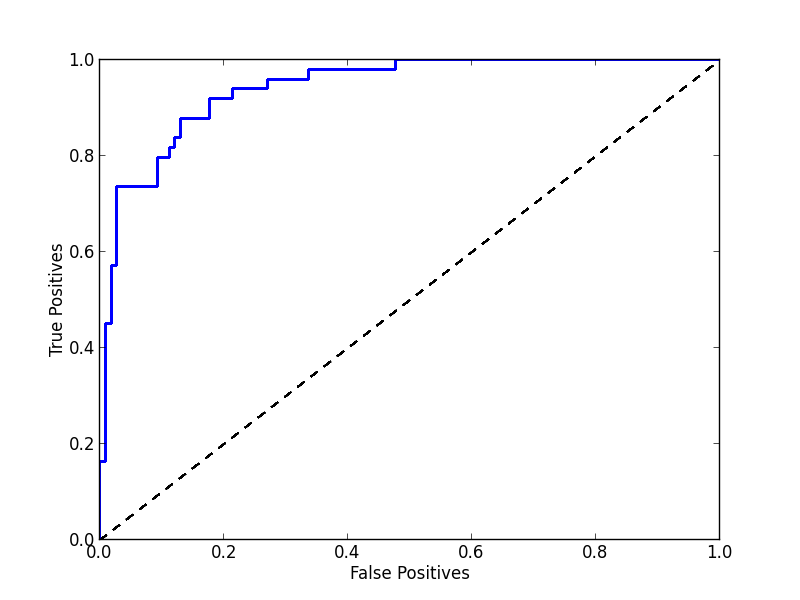
\includegraphics[width=0.65\textwidth]{images/testing/ROC.png}
\caption{ ROC Curve for Partridge's Random Forest Topic Classifier}
\label{fig:roc_random_forest}
\end{center}
\end{figure}

\subsection{ Area Under Curve }

The Area Under the Curve (AUC) measure is calculated as a percentage of  the
area underneath a ROC curve. This can again be used to give an indication of
the trade-off between true positive and false positive classification. It is a
percentage measurement, where 100\% indicates a high TP-FP ratio. AUC is often
used instead of visualising a ROC graph for brevity or where average
performance of a classifier over several train-test cycles is to be calculated.
The average AUC for Partridge's Random Tree Paper Type classifier after is
96.6\% after three fold validation is executed over the whole set of papers.

Comparison of this result with the above graph does show discrepancies between
simple 60:40 proportional validation and 3-fold validation - the average
performance of the latter seems to be slightly more accurate. This may be
because a slightly higher number of training examples (66\% rather than 60\%)
were used to train the classifiers during 3-fold validation and that the errors
were averaged out at the end of the process.

\subsection{ Confusion Matrices}

Confusion Matrices are a way of showing comprehensively which classes a machine
learning system struggles to discriminate between the most. Known classes are
shown on the vertical axis of the matrix and predicted classes are shown across
the horizontal. This allows inference of which data classes a trained
classifier struggles to label most frequently and any classes that it commonly
confuses them with. A set of confusion matrices for the Paper Type Classifier
in Partridge can be seen in Figure \ref{fig:conf_matrices} below.

\begin{figure}[!h]

\centering

\begin{subfigure}[b]{\textwidth}

\caption{Fold 1 Results}
\centering
\begin{tabular}{ | r l l l l |}
\hline
\multirow{5}{*}{\begin{sideways}{Actual Class}\end{sideways}}
&&\multicolumn{3}{c|}{Predicted Class} \\
&& \multicolumn{1}{c}{Case Study} &	Research&	\multicolumn{1}{c|}{Review}\\
\cline{3-5}
& \multicolumn{1}{c|}{Case Study} &	83&		2&		12\\
&\multicolumn{1}{c|}{Research}&	3&		255&		0\\
&\multicolumn{1}{c|}{Review}&	4&		2&		159\\
\hline

\end{tabular}
\end{subfigure}


\begin{subfigure}[b]{\textwidth}

\caption{Fold 2 Results}
\centering
\begin{tabular}{ | r l l l l |}
\hline
\multirow{5}{*}{\begin{sideways}{Actual Class}\end{sideways}}
&&\multicolumn{3}{c|}{Predicted Class} \\
&& \multicolumn{1}{c}{Case Study} &	Research&	\multicolumn{1}{c|}{Review}\\
\cline{3-5}
&\multicolumn{1}{c|}{Case Study}&   85    &         2&		10\\
&\multicolumn{1}{c|}{Research}&	0   &		256&		2\\
&\multicolumn{1}{c|}{Review}&	5&		1&		159\\
\hline
\end{tabular}

\end{subfigure}

\begin{subfigure}[b]{\textwidth}

\caption{Fold 3 Results}
\centering
\begin{tabular}{ | r l l l l |}
\hline
\multirow{5}{*}{\begin{sideways}{Actual Class}\end{sideways}}
&&\multicolumn{3}{c|}{Predicted Class} \\
&& \multicolumn{1}{c}{Case Study} &	Research&	\multicolumn{1}{c|}{Review}\\
\cline{3-5}
&\multicolumn{1}{c|}{Case Study}&	82&		3	&	12 \\
&\multicolumn{1}{c|}{Research}&	0&		257	&	1\\
&\multicolumn{1}{c|}{Review}&		7&		2	&	156\\
\hline
\end{tabular}

\end{subfigure}

\caption{ Confusion matricies for the 3-Fold validation process}
\label{fig:conf_matrices}

\end{figure}

These results show that Partridge's decision tree is very effective at
classifying the three document types in its database. It is also clear however,
that whilst the classifier is outstanding at recognising Research papers, it
sometimes struggles to discriminate between Case Study and review papers. This
may be because case studies can be considered a specific type of review paper
and the two classes share more similar CoreSC features than they do with
research papers.  

\subsection{ Precision, Recall and F-Measure }

From a classifier's confusion matrices, it is possible to calculate its
Precision, Recall and F-Measure values. These can be used to make further
assertions about the validity of a classifier's behaviour
\cite{witten2005data}.

The Precision of a classifier is the fraction of data samples retrieved that
were correctly classified. This is defined as:
\[Precision = \frac{tp}{tp+fp} \]

The Recall of a classifier is the proportion of samples within a given class
that the classifier is able to correctly classify. For example: the number of
apples that a classifier identifies as apples within a training set of fruit.
This is defined as:
\[Recall = \frac{tp}{tp+fn} \]

The F-Measure of a classifier is used to characterise both Recall and Precision
in a single value. The F-Measure of a classifer can be defined as:
\[
F-Measure = \frac{ 2 \times Recall \times Precision} { Recall + Precision } = 
\frac{2 . TP}{ 2 . TP + FP + FN }
\]


\begin{figure}[!th]

\centering
\begin{tabular}{| l | l | l | l | l |}
\hline
&        &\textbf{Recall}&\textbf{Precision}&\textbf{F-Measure}\\
\hline
\hline
\multirow{4}{*}{Fold 1} & Case Study & 0.85 & 0.92 & 0.89 \\
                        & Review     & 0.96 & 0.92 & 0.94 \\
                        & Research   & 0.98 & 0.98 & 0.98 \\
\hline

\multirow{4}{*}{Fold 2} & Case Study & 0.87 & 0.94 & 0.91 \\
                        & Review     & 0.96 & 0.92 & 0.94 \\
                        & Research   & 0.99 & 0.98 & 0.99 \\

\hline

\multirow{4}{*}{Fold 3} &Case Study & 0.84 & 0.92 & 0.88 \\
                        & Review    & 0.95 & 0.92 & 0.93 \\
                        & Research  & 0.99 & 0.98 & 0.99 \\


\hline


\end{tabular}

\caption{Recall Precision and F-Measure values for Partridge Topic Classifier}
\label{fig:fmeasure_table}

\end{figure}

Recall, Precision and F-Measure was calculated for each of the classes and in
each iteration of the three fold validation sequence. The results in Figure
\ref{fig:fmeasure_table} show good recall, precision and f-measure for all
three document types within Partridge. These results verify that Case Study is
the hardest document type to classify as discussed above.

\section{ User Testing } 

Raymond(1999) suggests that for developers of open source projects, ``Treating
your users as co-developers is your least-hassle route to rapid code
improvement and effective debugging\cite{raymond1999cathedral}." Partridge
hasn't been developed using an open methodology since, as a dissertation
project, it has been necessary to avoid complications around work ownership.
However, Raymond's notion that software should be released early and often and
tested on its user-base is an effective one and has been widely adopted by both
open and closed source developers\cite{linux2013}\cite{unity2013}.

A publicly available instance of Partridge that can be accessed at
(\url{http://farnsworth.papro.org.uk/}) was made available as soon as iteration
1 was complete and advertised using several social media streams. This was an
effort to attract as many users to Partridge as possible in the early stages of
the project in order to provide user testing. It was made clear to any early
adopting users that the system was still in development and they were
encouraged to submit bug reports if they experienced any problems whilst using
the site. This was a great success and a number of bugs and suggested
improvements were raised both via the GitHub repository and in conversation,
helping to improve Partridge and find some defects that had previously been
overlooked. For example, one user noticed that the full text search within
Partridge was not behaving as expected and returning all papers regardless of
their contents.  The relevant code was repaired and the bug marked as resolved
on GitHub\cite{softlybug2013}.


\subsection{Intrinsic Feedback} 

Intelligent information retrieval using machine learning techniques is a
complicated and multifaceted process. Partridge attempts to encode this complex set of
procedures into a usable and understandable interface designed for the use of
non-programmers. It was therefore important to understand how usable the
interface is for non-technical users.

Most users who commented on the system found that the query form made a lot of
sense and helped them to identify relevant papers very quickly. 

There were a few comments on how the uploader system could be improved. Users
were confused by the preprocessor and wondered why their paper didn't appear in
the corpus as soon as they submitted it. The most popular solution to this was
to add an email field to the uploader so that people who submit papers to the
corpus are notified when their paper is incorporated. This also provided
feedback for users whose papers could not be added to the corpus due to errors
or rights ownership issues.

Another suggestion was to add a twitter bot to announce when new papers have
been added to the system. This would provide another way of issuing user
feedback when a paper is submitted and would also help to draw users to
Partridge - especially when high profile papers are successfully added to the
system.

\subsection{Extrinsic Feedback}

As well as finding out how Partridge performs as a system, it was interesting
to find out how Partridge blended in to the information retrieval ecosystem around
it and how effectively it could be used day to day or in combination with any other
online tools.

One of the most important suggestions made was the addition of the Bookmarklet
tool. This had the effect of making paper submission to Partridge a lot more
convenient and intuitive. It also helped reduce confusion over paper
rights since the bookmarklet only works on sites which license
their papers under permissive licenses and allow data mining. 

\section{Summary}

The extensive range of testing methodologies used throughout the project meant
that Partridge has been developed into a mature, stable and highly usable
product. Unit testing has ensured that all procedural and scripted
functionality within Partridge is predictable and reliable. Machine Learning
Evaluation has ensured that an accurate and precise paper type classification
mechanism has been developed and User Testing has ensured that non-technical
users are able to use Partridge effectively.

Testing has been highly effective throughout the project and any potential
issues with the system were identified very early on and resolved due to the
`open-source-esque' development lifecycle used during the project.  Testing has
also provided a great deal of understanding about just how useful Partridge is
as well as highlighting its limitations. It also raises questions as to the
future development of the project and provides a number of ideas for future
improvements.
